\documentclass[border=10pt]{standalone}
\usepackage{tikz}
\usetikzlibrary{arrows.meta, decorations.pathmorphing}

\begin{document}

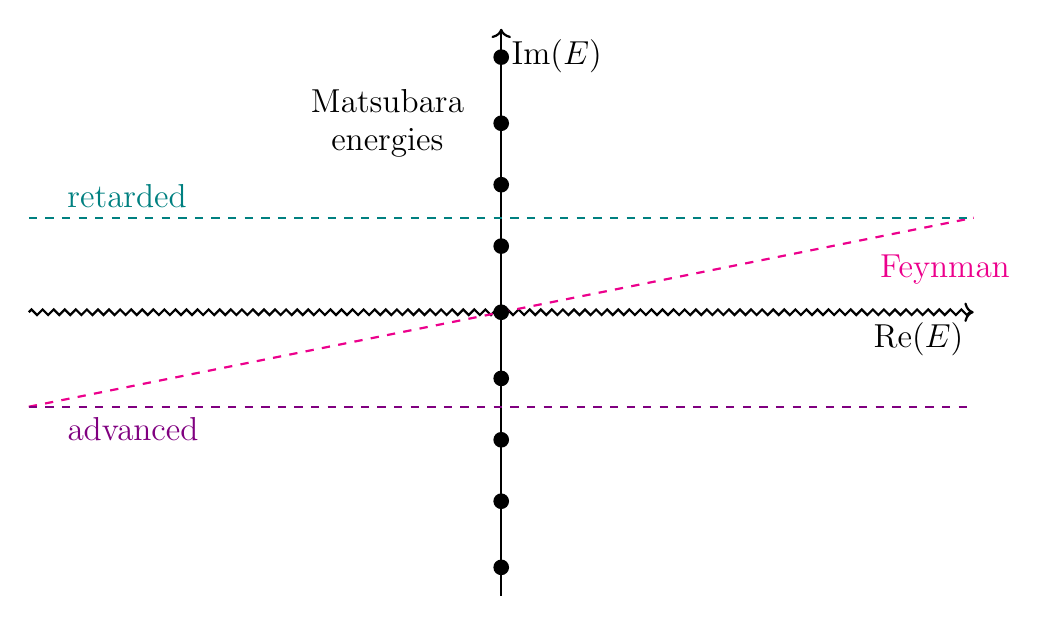
\begin{tikzpicture}[
    scale=1.2,
    every node/.style={font=\large},
    axis/.style={->, thick},
    matpoint/.style={fill, circle, inner sep=2pt},
    feynman/.style={dashed, magenta, thick},
    retarded/.style={dashed, teal, thick},
    advanced/.style={dashed, violet, thick},
    wavy/.style={decorate, decoration={zigzag, amplitude=1pt, segment length=4pt}, thick}
]

% Axes
\draw[axis] (0, -3) -- (0, 3) node[below right] {$\mathrm{Im}(E)$};
\draw[axis, wavy] (-5, 0) -- (5, 0) node[below left] {$\mathrm{Re}(E)$};

% Label for Matsubara energies
\node[align=center, left=10pt] at (0, 2) {Matsubara\\energies};

% Feynman propagator (dashed magenta line with positive slope)
\draw[feynman] (-5, -1) -- (5, 1);
\node[feynman, right] at (3.9, 0.45) {Feynman};

% Retarded propagator (horizontal teal dashed line above real axis)
\draw[retarded] (-5, 1) -- (5, 1);
\node[retarded, above right] at (-4.7, 1) {retarded};

% Advanced propagator (horizontal purple dashed line below real axis)
\draw[advanced] (-5, -1) -- (5, -1);
\node[advanced, below right] at (-4.7, -1) {advanced};

% Matsubara energies (discrete points on Im axis)
\foreach \y in {-2.7, -2, -1.35, -0.7, 0, 0.7, 1.35, 2, 2.7} {
    \node[matpoint] at (0, \y) {};
}

\end{tikzpicture}

\end{document}
